


\tableofcontents

%\emptypage
\newpage

\chapternonum{Introduction}

%==============================================================
\chapter{The Standard Model of particle physics and beyond}
%==============================================================

    \section{Fields and symmetries}

        \subsection{Quantum field theory and feynman diagrams}


	While the topic of interest here is the physics of particles, one should 
    never forget about the underlying structure behind them : fields. A field 
    is a physical quantity defined across space and time. Relative quantum 
    field theory is a theoretical framework which was developed during the 
    twentieth century and allowed to unify quantum mechanics and special 
    relativity.

	In such a field theory, particles are excitations of the fields (of field 
    quanta) and interactions refers to coupling terms between those fields. 
    In a sense, the goal of a particle physicist can be seen as using particles
    as a mean to understand which fields exists, what are their properties and
    how they couple with each other.

    Quantum field theory makes use of the Lagrangian formalism. In particular, 
    the Lagrangian function $\mathcal{L}$ is a core element as it allows to 
    summarize the dynamics of a system in an elegant and concise way. This 
    function depends of the fields $\phi(t,x)$ and their derivatives with 
    respect to time and space. One can obtain the equation of motion from it 
    by using the Euler-Lagrange equation :

    $$
        \frac{\partial \mathcal{L}}{\partial \phi} 
        - 
        \frac{\partial}{\partial x^\mu} 
        \left( 
            \frac{\partial \mathcal{L}}{\partial (\partial \phi / \partial x^\mu)} 
        \right) 
        = 
        0
    $$

    An interesting feature of the Lagrangian is that terms that are a product
    of three of more fields corresponds to an interaction between these fields.
    For instance in the simple case with three scalar fields $\phi_{i,\ i = 1,2,3}$, 
    a term $k \cdot \phi_1 \phi_2 \phi_3$ corresponds to a coupling between those
    fields with a strength $k$. 
    
    There is also a direct correspondance between such a term and an interaction 
    vertex which can be represented using Feynman diagram. Feynman diagrams are 
    graphical representations of the evolution of a system of particles where 
    interactions occur. Though there is no general convention about the orientation 
    of space and time when drawing such a diagram, this document will always 
    represent space along the horizontal axis and time evolving from left to right.
    Feynman diagrams provides an intuitive understanding of a physical process but 
    also a mathematical tool to compute probility amplitude for a transition between 
    an initial state and a final state using Feynman rules.

    \insertFigure{feynmanDiagramExample}{0.3}
                 {Example of vertex corresponding to a Lagrangian term $k \cdot \phi_1 \phi_2 \phi_3$.}

        \subsection{Noether's theorem and symmetries}
        \loremipsum

    \section{The Standard Model of particle physics}
        \subsection{The strong sector}
        \loremipsum
        \subsection{The electroweak sector}
        \loremipsum
        \subsection{The electroweak symmetry breaking}
        \loremipsum

    \section{Limitations of the Standard Model}
        \subsection{Open questions and criticism}
        \loremipsum
        \subsection{The hierachy problem}
        \loremipsum
        \subsection{The dark matter}
        \loremipsum

    \section{Theories beyond the Standard Model}
        \subsection{Zoology of Standard Model extensions}
        \loremipsum
        \subsection{Supersymmetry}
        \loremipsum
        \subsection{Constrains on top partners and dark matter}
        \loremipsum
            \subsubsection{Cosmology}
        \loremipsum
            \subsubsection{Particle physics}
        \loremipsum











%==============================================================
\chapter{The Compact Muon Solenoid experiment at the LHC}
%==============================================================

    \section{The Large Hadron Collider}
        \loremipsum
        \subsection{Scientific context and program}
        \loremipsum
        \subsection{Setup}
        \loremipsum
        \subsection{Performances during Run I}
        \loremipsum

    \section{The Compact Muon Solenoid experiment}
        \loremipsum
        \subsection{The CMS detector}
        \loremipsum
            \subsubsection{The tracker and magnet}
        \loremipsum
            \subsubsection{The calorimeters}
        \loremipsum
            \subsubsection{The muon chambers}
        \loremipsum
        \subsection{Trigger system}
        \loremipsum
            \subsubsection{L1}
        \loremipsum
            \subsubsection{HLT}
        \loremipsum
        \subsection{Object reconstruction algorithms and calibration}
            \subsubsection{Vertex and tracks}
        \loremipsum
            \subsubsection{Electrons and photons}
        \loremipsum
            \subsubsection{Muons}
        \loremipsum
            \subsubsection{Jets and missing energy}
            %(maybe plot showing the difference of jet clust algorithm for a same event/example)
        \loremipsum
        \subsection{Performances}
        \loremipsum
            \subsubsection{Particle-flow vs Calo-based algorithm ?}
        \loremipsum
            \subsubsection{Expected vs current performances ?}
        \loremipsum
            \subsubsection{Upcoming upgrades ?}
        \loremipsum

     \section{Monte Carlo generator and detector simulation}
        \loremipsum
        \subsection{Hard scattering}
        \loremipsum
        \subsection{Parton showering}
        \loremipsum
        \subsection{Detector simulation}
        \loremipsum

%==============================================================
\chapter{b-tagging techniques in CMS}
%==============================================================

    \section{Principle and importance of b-tagging techniques}
        \loremipsum

    \section{Discriminating observables and algorithms}
        \loremipsum
        \subsection{Impact parameter}
        \loremipsum
        \subsection{Secondary vertex}
        \loremipsum
        \subsection{Soft leptons}
        \loremipsum
        \subsection{Track counting algorithm}
        \loremipsum
        \subsection{Simple secondary vertex}
        \loremipsum
        \subsection{CSV}
        \loremipsum

    \section{Algorithms performances and prospectives}
        \loremipsum
        \subsection{Performances at 8 TeV}
        \loremipsum
        \subsection{Expected performances for Run II}
        \loremipsum
        \subsection{Development of boosted algorithms}
        \loremipsum
        \subsection{Studies for high PU conditions}
        \loremipsum







%==============================================================
\chapter{Search for stop pair production at $\sqrt{s}$ = 8 TeV}
%==============================================================

    This chapter focuses on an analysis performed within the CMS collaboration 
    and searching for the production of stop pair using the data recorded during 
    the Run I of the LHC at $\sqrt{s}$ = 8 TeV. In section \ref{sec:analysis_contextAndPheno}, 
    we concentrate on the context and phenomelogy of the signature while section 
    \ref{sec:analysis_objectAndEventSelection} to \ref{sec:analysis_results} discuss 
    the different aspects of the analysis itself and the results. In the last sections 
    \ref{sec:analysis_perspective} and \ref{sec:analysis_overviewStopSearches}, some 
    of the perspectives for this analysis are presented, as well as an overview of 
    other top-partner searches within the CMS collaboration.

    \section{Context and phenomenology \label{sec:analysis_contextAndPheno}}

        \subsection{Theoretical context and assumptions}

        One of the best assets of supersymmetry is its ability to solve the hierarchy 
        problem in a natural way, that is by requiring a small amount for fine-tunning 
        to explain the low mass of the Higgs Boson. In particular, the top quark $t$ 
        contribution to the divergence of the Higgs is reduced by the introduction of 
        the stop quark $\lstop$ \todo{illustration}. In the simplest case, the two 
        contributions would cancel each other perfectly provided that the top and stop 
        quarks have the same mass. However, it has been experimentally shown that this 
        is not the case \todo{reference, justification ?}. Nevertheless, naturalness can 
        be used to constrain the stop mass if ones define what is an acceptable level of 
        tunning. Despite the fact that such constrain is highly dependent of hypothesis
        made on the SUSY parameters, it is commonly admitted that stop quarks should have
        a mass below or around 1 TeV for SUSY to remain natural. This makes the search
        for stop and important channel for possible SUSY discovery.

        A second appealing feature of supersymmetry is that it can provide a dark matter 
        candidate. This happens in R-parity conserving models where the lightest supersymmetric
        particle (LSP) is a natural WIMP candidate if it is not a charged particle. In the
        context of the MSSM, the lightest neutralino $\lneutralino$, the gravitino $\tilde{G}$
        and the lightest sneutrino $\tilde{\nu}$ can be the LSP and therefore are dark matter
        candidate. The lightest neutralino is the one that is most often studied. Neutralinos
        $\tilde{\chi}$ are combination of the bino $\tilde{B}$, the two neutral higgsinos 
        $\tilde{H}_{1,2}$, and the neutral wino $\tilde{W}_3$. One can compute the relic
        abudance of dark matter by solving the Boltzmann equation \cite{EllisDarkMatter}
        depending essentially of the LSP mass $m_{\text{LSP}}$ and the annihilation cross-section.
        The next-to-lightest supersymmetric particle (NLSP) mass is a crucial parameter as 
        it strongly affect the annihilation cross-section and therefore the relic abudance. 
        In particular, cosmological observations are favorizing cases where the LSP is 
        degenerated with the lightest stop $\lstop$ or stau $\tilde{\tau_1}$.
        
        These two considerations lead to a logical interest in phenomenology where both a 
        neutralino LSP and a light stop NLSP have relatively low mass and accessible at the LHC.

        \subsection{Phenomenology and signature}

        In this subsection, we focus on presenting the targetted process of the search discussed 
        in sections \ref{sec:analysis_objectAndEventSelection} to \ref{sec:analysis_results} and 
        its phenomenology. As it is in practice impossible to scan the whole phase space of SUSY
        models, a pragmatic approach often consist in using simplified SUSY models where an 
        effective lagrangian is introduced to consider a limited set of new physics features. 
        This has the advantage of producing generic interpretations of experimental searches, 
        making it possible to reinterpret them in specific realization of SUSY \cite{SusySimplifiedModels, SmodelS}.

        In our case, we consider the lightest stop $\lstop$, the lightest neutralino 
        $\lneutralino$ and allow the stop to decay through $\lstop \rightarrow t \lneutralino$. 
        It introduces two new parameters which are the masses of the new particles, $\mass{\lstop}$ 
        and $\mass{\lneutralino}$. This is represented on figure \ref{fig:stopDecayModes} on the left. 
        This decay mode is refered to as $T2tt$ in the simplified model nomenclature. In addition, 
        we also consider the case where the lightest chargino with a mass $\mass{\lchargino}$ such 
        as $\mass{\lstop} > \mass{\lchargino} > \mass{\lneutralino}$ and stop decay through the 
        chain $\lstop \rightarrow b \lchargino \rightarrow b W^{\pm} \lneutralino$. We introduce 
        $x$ such as $\mass{\lchargino} = x \cdot \mass{\lstop} + (1 - x) \cdot \mass{\lneutralino}$ 
        and study the three cases $x = 0.75$, $0.50$ and $0.25$ as described on figure \ref{fig:stopDecayModes} 
        on the right. This decay mode is refered to as $T2bw$ in the simplified model nomenclature. 
        All of these four signal types are studied independently of each other with a branching ratio 
        equal to 1.

        \insertFigure{stopDecayModes}{0.8}
                     {Representation of the mass hierarchy in the $\lstop \rightarrow t \lneutralino$ 
                     decay mode (on the left) and $\lstop \rightarrow b \lchargino \rightarrow b W^{\pm} 
                     \lneutralino $ decay mode (on the right). For the later, the chargino mass $\mass{\lchargino}$ 
                     is parametrized using $\mass{\lchargino} = x \cdot \mass{\lneutralino} + (1 - x) \cdot \mass{\lstop}$ 
                     and three different values of $x$ will be studied, $x = 0.75$, $0.50$ and $0.25$.} 
    
        Here, our interest is in the case where a stop pair is produced during a $pp$ collision, 
        as represented in the Feynman diagrams of figure \ref{fig:stopFeynmanDiagrams}. One should 
        notice that it is relevant to study the two type of decay modes together as, considering 
        that the top quark almost exclusively decays through $t \rightarrow b W^+$, they lead to 
        the same intermediate state $b \bar{b} W^+ W^- + \lneutralino \lneutralino$. Each of the 
        $W$ bosons can then decay either hadronically, into a quark pair ($W \rightarrow q\bar{q}$), 
        or leptonically, into a lepton and a neutrino ($W \rightarrow \ell \nu_{\ell}$). If the two 
        $W$ bosons decay hadronically, the final state is said to be fully hadronic, or 0-lepton. 
        In the case where one of the $W$ bosons decays hadronically and the other leptonically, the 
        final state is said to be semi-leptonic, or 1-lepton. Finally, if the two $W$ bosons decay 
        leptonically, the final state is said di-leptonic or 2-leptons. The search performed in this 
        thesis focus on the 1-lepton channel. 

        \insertTwoFigures{stopFeynmanDiagrams}
                         {feynmanDiagram_T2tt}{feynmanDiagram_T2bw}{0.4}
                         {Feynman diagrams of stop pair production in $pp$ collisions for the 
                         $\lstop \rightarrow t \lneutralino$ decay mode (on the left) and 
                         $\lstop \rightarrow b \lchargino \rightarrow b W^{\pm} \lneutralino$ decay mode 
                         (on the right). The lines of the supersymmetric particles are drawn in red.}
   
        As the $\lneutralino$ are assumed to be dark matter candidates, they do not interact with the 
        detector. Therefore, the signature left by this new physic process is the production of two top 
        quarks associated with extra missing transverse energy coming from the two $\lneutralino$. The 
        search is performed for several benchmarks across the $(\mass{\lstop},\mass{\lneutralino})$ plane 
        represented on Figure \ref{fig:stopMassSpace}. A key phenomenological feature is the way that the 
        momentum carried by the decay products strongly depends of $\deltam \definedAs \mass{\lstop} - \mass{\lneutralino}$.
        This affects both the missing transverse energy and the momentum of jets and leptons in the final
        state. As a result, it will be easier to differentiate between the standard model background and 
        a signal with high $\deltam$ compared to lower $\deltam$. The Figure \ref{fig:phenoT2tt} present
        the illustrate the evolution of the mean generated $MET$ and top $p_T$ as function of $(\mass{\lstop},
        \mass{\lneutralino})$. The most challenging scenario happens for the $\lstop \rightarrow t \lneutralino$
        decay mode when $\deltam = \mass{t}$, since the signal kinematic remains close to the standard
        model $t\bar{t}$ production in that case. One can also consider signal involving an off-shell
        top quark or W boson in the $\lstop \rightarrow t \lneutralino$ or $\lstop \rightarrow b \lchargino$
        decay modes respectively.

    \insertTwoFigures{stopMassSpace}
                     {massSpace_T2tt}{massSpace_T2bw}{0.49}
                     {Mass space of the stop pair production search for the $\lstop \rightarrow t \lneutralino$
                     decay mode (on the left) and $\lstop \rightarrow b \lchargino \rightarrow b W^{\pm} \lneutralino $
                     decay mode (on the right). The blue dashed lines represent the limit for the off-shell topology.
                     The grey part is not kinematically allowed.}
 
    \insertTwoFigures{phenoT2tt}
                     {phenoT2tt_meanGenMET}{phenoT2tt_meanGenTopPt}{0.45}
                     {Evolution of the mean generated missing tranverse energy (on the left) and top $\pT$
                     (on the right) for the $\lstop \rightarrow t \lneutralino$ decay mode. A selection requiring
                     at least one high-$\pT$ central electron or muon and at least three high-$\pT$ central jets
                     has been applied.}

    \section{Objects and events selection \label{sec:analysis_objectAndEventSelection}}

    This section focuses of the first aspect of the experimental search, namely the object and event selection. 
    The goal here is to first, present the criteria used to define the objects in the context of this analysis,
    and second, the baseline event selection based on the signature being looked for.

        \subsection{Trigger}

    \todo{reference (TRG legacy paper?)}
    
    This search uses mainly single lepton triggers. The single muon trigger requires an isolated muon candidate
    with $\pT > 24 \GeV$ and a relative isolation lower than 15\% in a cone of 0.3. The single electron trigger
    requires an electron candidate with $\pT > 27 \GeV$ along with quality criteria applied on the shower shape,
    the matching between track and supercluster, and ratio between hadronic and electromagnetic energy, such that
    the resulting efficiency is about 80\%.

    In addition of the single muon and electron trigger, a muon+jets trigger is used, allowing a lower $\pT$ treshold
    for the muon. This trigger requires a muon candidate with $\pT > 17 \GeV$ and $\abseta < 2.1$ and at least three 
    jets with $\pT > 30 \GeV$ and $\abseta < 3.0$.

    Finally, the analysis also makes use of dilepton triggers for dilepton control regions. For these, electrons
    candidates are identified using loose requirements on the isolation and information from tracker and calorimeters.
    The leading lepton must have $\pT > 17 \GeV$ while the second lepton must have $\pT > 8 \GeV$.

        \subsection{Leptons}

        After full reconstruction of the events, further criteria are applied on the lepton candidates 

            \subsubsection{Selected leptons}

        Electron candidates are requested to have $\pT > 30 \GeV$ and $\abseta < 1.4442$ and good vertex compatibility,
        low number of missing hits and low amount of radiation in the tracker using the medium identification working point
        of the collaboration \todo{reference}. Muon candidates are requested to have $\pT > 20 \GeV$ and $\abseta < 2.1$
        and good vertex compatibility, good fit quality for the track and a minimum number of hits in both the tracker
        and the muon subdetectors using the tight identification working point of the collaboration \todo{reference}.

        For both muons and electron, a relative isolation is computed inside a cone of $\Delta R = 0.3$ around the lepton.
        The isolation is computed using the particle-flow information by summing the $p_T$ of charged particles inside
        the cone, as well as neutral particles for which the pile-up density is substracted using the effective-area 
        scheme for electrons and $\Delta \beta$ scheme for muons. The relative isolation is required to be lower than
        15\% while the absolute isolation is required to be lower than $5 \GeV$.

        \subsubsection{Veto leptons \label{sec:vetoLeptons}}

        As it will be seen in section \ref{sec:analysis_optimization}, the dileptonic $t\bar{t}$ process becomes a major
        background of this analysis after cutting on the variable $\MT$. This motivates the development of efficient ways
        to reject this specific background : in particular, the development of a veto targeting events with a second, lost 
        lepton.

        The first category of veto lepton targets an isolated track left by a second electron or muon, or by a tau hadron
        decaying into only one charged hadron (one prong). To do this, we look for a reconstructed charged particle in the
        event. \todo{criteria}

        The second category of veto lepton targets a tau lepton that decayed hadronically into one or more charged hadron.
        \todo{fill the rest}

        \todo{performance : breakdown matrix of second lepton category vs evolution as function of cuts in second lepton vetos}

        \subsection{Jets and missing transverse energy}

       Jets are reconstructed using the anti-$k_t$ clustering algorithm with a parameter $R = 0.5$ on the particle-flow
       information. Three types of corrections are applied : an energy offset an $\eta$ dependent and $p_T$ dependent
       corrections, as well as a residual correction accounting for discrepancies between data and simulation.

       Selected jets are required to have $p_T > 30 \GeV$ and $\abseta < 2.4$. They also have to be separated from
       lepton candidates in $\Delta R > 0.4$ and to pass a jet identification criteria \todo{reference} with loose
       requirements on the neutral and charged fractions, charged multiplicity and number of constituents. Furthermore,
       a pile-up identification algorithm is used which combine the vertex compatibility, the topology of the jet shape 
       and the jet object multiplicity \todo{reference}.

       $b$-tagged jet are defined by, on top of the previous requirements, using the medium working point of the 
       Combined Secondary Vertex (CSV) tagging algorithm. \todo{Mention efficiency and fake rate}

       The value of the CSV discriminant is corrected in the simulation as function of the $p_T$ and $\eta$
       of the jet to account for known data/MC discrepancies.

       The missing transverse energy is computed by considering the negative vector sum of jets, leptons and 
       unclustered particles reconstructed by the particle-flow algorithms. It is corrected by propagating the 
       corrections applied on the jets. An other correction allows to remove a modulation along $\phi$, observed 
       in both data and simulation.

        \subsection{Events selection}

        The baseline selection, or preselection, is defined by asking exactly one electron or muon, at least 
        four jets among which at least one is $b$-tagged, and a missing transverse energy higher than $80 \GeV$.
        A veto is applied on events containing a second lepton as defined in \ref{sec:vetoLeptons}. Additionally,
        we filter events that are known to suffer from noise or anomalous subdetector operation, as well as events
        with inconsistent directions of the missing transverse energy calorimeter-based and particle-flow-based
        approach ($\Delta \phi < 1.5$). For data, we require that events with a leading electron fired the single
        electron trigger, while for events with a leading muon, the cross-trigger has to be fired if the muon $\pT$
        is within $\left[ 20, 26 \right] \GeV$ otherwise the single muon trigger is used.

        \todo{detail background category, mention that only those with significant contribution are shown,
        for instance QCD is ignored because suppressed by MET cut}

        \todo{cutflow table}
        
        \todo{plot showing signal selection efficiency}
        
    \section{Signal region design and optimisation \label{sec:analysis_optimization}}

    After the baseline selection, the two dominant background categories are the $\oneLeptonTop$
    and $\Wjets$. For both of these backgrounds, the only main source of missing energy is a neutrino
    coming from the leptonic decay of a $W$ boson, $W \rightarrow \ell \nu_{\ell}$. In comparison,
    the signal has three main sources of missing energy. One can exploit this difference by noticing
    that for the background, the transverse mass of the ($\ell$,$\vec{MET}$) system has a kinematic
    end at $\mass{W} \sim 80 \GeV$, while the same variable can get to higher values for the signal.
    We therefore introduce the variable $\MT \definedAs \sqrt{2 \left|\vec{MET}\right| \pT^\ell ( 1 - cos( \Delta \phi  ) ) }$
    where $\Delta \phi$ is the azimuthal angle between the lepton and the $\vec{MET}$ directions.

    Figure \ref{fig:MTatPreselection} shows how $\MT$ distributes for the different backgrounds and
    two signal examples after preselection. Given the discriminating power that this variable provides,
    cutting on it is the starting point of all the signal region definitions following. The base cut
    applied is $\MT > 100 \GeV$. Table \ref{tab:MTcutImpact} shows a quantitave breakdown of the impact
    of the cut on the different yields. In particular, one can notice how the $\diLeptonTop$ fraction increases.

    \insertTwoFigures{MTatPreselection}
                     {MTsuperimposed}{MTstack}{0.45}
                     {Distribution of $\MT$ for the different backgrounds and two signal examples,
                     superimposed after normalization to one (on the left) or stacked after normalization to the luminosity (on the right).}

        \todo{cutflow table showing impact of MT cut}

        \subsection{Discriminating variables}

        To further increase the signal-to-noise ratio, several signal regions are constructed to adress
        specific regions of the $(\mass{\lstop},\mass{\lneutralino})$ space. These regions are designed
        by considering other discriminating variables. Two approaches are considered : a cut-based approach
        that consist of a list of cuts on variables, and a boosted decision tree approach that combines
        multiple inputs into one discriminating variable on which a cut is applied. We first present the
        variables that are considered, with an attempt to classify them according to their nature.

           \subsubsection{Kinematic and angular variables}

                \begin{itemize}
                    \item $p_T(\ell)$, $p_T(\text{lead. jet})$, $p_T(\text{lead. } b)$ ;
                    \item $H_T$ ;
                    \item $\Delta R( \ell, \text{lead. } b)$ ;
                \end{itemize}

           \subsubsection{Missing energy related and topology}

                \begin{itemize}
                    \item  $MET$ ; while the preselection already includes a cut on the missing
                        transverse energy, cutting further on it can significantly increase the
                        signal-to-noise ratio, especially at high masses.
                    \item  $MET / \sqrt{H_T}$ ; an alternative to $MET$ is the use of $MET / \sqrt{H_T}$.
                        Cutting on this variable can be interpreted as a two-dimensional cut using
                        the formula $MET^{2} < k^2 \cdot H_T$ where $k$ is the value of the cut.
                        This allows to better reject background events with a high $MET$ value coming
                        from detector effect and uncertanty due to large hadronic activity in the event.
                    \item $\Delta \phi( j_{1,2}, \vec{MET} )$ ;
                    \item $H_{T}^\text{ratio}$ ;
                \end{itemize}

           \subsubsection{Invariant masses, kinematic fit}
           
                \begin{itemize}
                    \item $M_{T2}^{W}$ ;
                    \item Hadronic top $\chi^{2}$ ;
                    \item $M_{\ell b}$, $M'_{\ell b}$ ;
                    \item $M_{3b}$ ;
                \end{itemize}

           \subsubsection{Objects multiplicity}

                \begin{itemize}
                    \item Jet multiplicity ;
                    \item ISR-tagged jet ;
                \end{itemize}

            \todo{Finish variable description}

            \todo{Add sketches}

            \todo{Plots of shape for all / some variables ?}

            \subsection{Figure of merit}

            Before going into the details of the signal region optimization, we first need to introduce the
            metric used to do so. The problem of defining cuts to be applied on a variable can be summarized 
            as knowing how to compromise between the quantity of selected signal, $S(\text{cut})$, versus selected
            background, $B(\text{cut})$, such that the sensitivity of the analysis is maximized. Ideally,
            one would run the full statistical interpretation using toy data. However, such a procedure 
            is often CPU intensive and not suitable for an iterative process. A more flexible way is
            to define a figure of merit (FoM) that approximate the statistical interpretation one is aiming
            to perform.

            Let's consider the background only hypothesis $H_0$, also called null hypothesis, and the 
            signal hypothesis $H_1$. These hypothesis are modeled by a probability density function (pdf) of 
            the number of events, as sketched on Figure \ref{fig:interpretation}.
           
            \insertFigure{interpretation}{0.7}
                         {Illustration of the modelization of the hypothesis $H_0$ and $H_1$.}

            From the point of view of excluding a signal, a simple approach consist in computing the type 
            II error (or probability to miss a signal) provided that $D$ events are observed in the
            data. Assuming that the pdf is gaussian, one can express the distance between $D$ and $H_1$ in terms 
            of standard deviations using $(\text{mean}(H_1) - D) / \sigma(H_1) = (S + B - D) / \sqrt{S+B}$.
            The figure of merit can be defined from considering the expected value of this quantity when assuming 
            a toy data equal to $B$, the mean realization of $H_0$ : $\text{FoM}_\text{exclusion} \definedAs S 
            / \sqrt{S+B}$. The same reasonning applies to the point of view of signal discovery, considering 
            the type I error (or probability of false discovery), leading to $\text{FoM}_\text{discovery}
            \definedAs S/\sqrt{B}$.

            The FoM described so far however takes only into account the statistical uncertainty on signal and 
            background but not the systematic aspects. To get a more realistic uncertainty, one can add to 
            $\sigma^2(H)$ a term $f^2 B^2$ where $f$ represents an estimate of the relative systematic uncertainty 
            on the background. Additionally, to work around issues where the remaining statistics becomes low and 
            cuts are not realistic anymore, we ignore cases where $S < 3$ or $B < 1$.

            \todo{Comment about Asimov Z}

        \subsection{Cut-based signal regions}

            \subsubsection{Optimization procedure}

            The variables are first classified by their individual discriminating power, estimated by taking the 
            maximum FoM achievable on a few signal benchmarks when scanning the possible cuts. The most 
            discriminating variables are $\MT$, $MET$, $MET/\sqrt{H_T}$ and $M_{T2}^{W}$, We also consider 
            $\Delta \phi(j_{1,2},\vec{MET})$, hadronic top $\chi^2$, $p_T(\text{lead. } b)$ and the presence of a
            5th, ISR jet. These variables have low discrimating power at preselection level but get useful after
            additional cuts on $\MT$, $MET$, $MET/\sqrt{H_T}$ and $M_{T2}^W$ depending of the $\deltam$ considered.

            On a few signal benchmarks, we perform a $n$-dimensionnal optimization of the cuts on these variables,
            though not cutting on both $MET$ and $MET/\sqrt{H_T}$ at the same time. 

            %mention that we add a scale factor to 1ltop et Wjets to take into account background estimation effects


            \subsubsection{Results and performances}

            

            \loremipsum

        \subsection{BDT-based signal regions}
        
            \loremipsum

    \section{Background estimation \label{sec:analysis_backgroundEstimation}}

        \subsection{Overview} 

        In this section, we focus on the estimation of the different background contributions. 
        Four kinds of control regions are defined by inverting some of the requirements of the
        preselection and signal regions, as illustrated on Figure \ref{fig:backgroundEstimationOverview}.
        Each of these aim to provide signal-free sectors in which to check how good is the modeling
        of the backgrounds by the Monte-Carlo and perform data-driven estimations.

            \insertFigure{backgroundEstimationOverview}{0.7}
                         {Overview of the control regions used in the background estimation method.}

        The $\MT$-peak control region is defined by looking at events satisfying $50 < \MT < 80 \GeV$
        instead of the signal region $\MT$ requirement. This control region is enriched in $\oneLeptonTop$
        and is used as a well-controled region in which to normalize the $\oneLeptonTop$, $\Wjets$ 
        and $\diLeptonTop$ as documented in \ref{sec:MTpeakNormalization}.
        
        The $0b\text{-tag}$ control region is defined by requiring no $b$-tagged jet in the event.
        This region is enriched in $\Wjets$ and $\oneLeptonTop$ and is used to control and correct 
        the tail of $\MT$ for these two components as described in \ref{sec:MTtailCorrection}.

        The $2\ell$ control region is defined by requiring exactly two selected leptons instead of
        one, and lowering the $MET$ cut to $50 \GeV$. Additionnally, to limit the contribution
        from Drell-Yan, we veto events where the invariant mass of the dilepton system, $\mass{\ell\ell}$,
        is such that $\left|\mass{\ell\ell} - m_{Z}\right| < 15 \GeV$. Finally, the $1\ell$+veto control 
        region is defined by requiring exactly one selected leptons and one lepton veto. This region 
        is intended to control the modeling of the second lepton veto. Both the $2\ell$ and $1\ell$+veto
        are being looked at on the whole $\MT$ range and are not used to derive scale factors but only 
        systematic uncertainties on the background as detailed in \ref{sec:background_systematics}.

        \todo{Add cutflow table of the dirrent control regions at preselection ?}

        \subsection{Background normalization in $\MT$-peak \label{sec:MTpeakNormalization}}

            The $\MT$-peak control region, defined as $50 < \MT < 80 \GeV$ is the first step of the
            background estimation method. It is used to normalize the $\oneLeptonTop$, $\Wjets$ and
            $\diLeptonTop$ components while the rare component is taken directly from Monte-Carlo.
            This normalization is done for each signal region individually, effectively allowing to
            absorb disagreements caused by cuts on not-so-well modeled variables and effect from jet
            energy scale, trigger efficiency and lepton identification efficiencies. 

            The normalization is done in two steps : first, a scale factor $\SFpre$ is
            computed before the application of the second lepton veto, substracting the rare component :

            \begin{equation}
                \SFpre \definedAs \left( \frac{N(\text{data}) - N(\text{rare})}{N(\oneLeptonTop) + N(\Wjets) + N(\diLeptonTop)} \right)
                \label{eq:SFpreDefinition}
            \end{equation}

            $\SFpre$ is used to normalize only the $\diLeptonTop$ component \todo{Maybe explain why it's done this way ?}. Another scale factor, $\SFpost$ is used after application of the second lepton veto, substracting the rare and the corrected $\diLeptonTop$ component :

            \begin{equation}
                \SFpost \definedAs \left( \frac{N(\text{data}) - N(\text{rare}) - \SFpre \times N(\diLeptonTop)}{N(\oneLeptonTop) + N(\Wjets)} \right)
                \label{eq:SFpostDefinition}
            \end{equation}

            At preselection level, $\SFpre$ and $\SFpost$ are equal to $(1.06 \pm 0.01)$ and $(1.05 \pm 0.01)$ respectively.

        \subsection{$\MT$-tail correction in the $0b$-tag region \label{sec:MTtailCorrection}}

        The $0b$-tag control region allows to control the tail of $\MT$ of the $\Wjets$ and $\oneLeptonTop$ components. Before looking at the tail, however, we start by normalizing the background in the $\MT$ peak of this control region, in a similar fashion as what is done in \ref{sec:MTpeakNormalization}. This is done by introducing $\SFnobtag$, used to normalize the $\Wjets$ and $\oneLeptonTop$ contributions :

        \begin{equation}
            \SFnobtag \definedAs \left( \frac{N(\text{data}) - N(\text{rare}) - N(\diLeptonTop)}{N(\oneLeptonTop) + N(\Wjets)} \right)
            \label{eq:SF0btagDefinition}
        \end{equation}

        At preselection level, $\SFnobtag$ is found to be $(0.99 \pm 0.01)$. After normalization to the peak, a clear disagreement in the tail of $\MT$ is observed for $\MT > 100 \GeV$ between the data and Monte-Carlo, as shown on \ref{fig:templateFit/MT_notCorrected}. This is an important point of the analysis as it means that the Monte-Carlo needs to be corrected to have a reliable prediction of the $\oneLeptonTop$ and $\Wjets$ in the $\MT$ tail. So far, the understanding of this disagreement comes from two source : first, the off-shell contributions of $\Wjets$ is underestimated by the simulation, and second, detector effects leads to a larger tail for the $\oneLeptonTop$ events.

        \insertFigure{templateFit/MT_notCorrected}{0.7}
                     {Data/MC comparison on the full $M_T$ distribution in the $0b$-tag control region at preselection level, after propagation of $\SFnobtag$. A clear discrepancy is visible for $\MT > 100 \GeV$.}

        A method is put in place to correct the discrepancy using a template fit to estimate separately the contribution of $\oneLeptonTop$ and $\Wjets$ from the data. To do this, we use $\MlbPrime$ which was found to have a good discriminating power between the two process categories and being well discribed in the peak of $\MT$, as shown on \ref{fig:MlbPrimeForTemplateFit}.

        \insertFourFigures{MlbPrimeForTemplateFit}
                          {templateFit/Mlb_0b_peak}
                          {templateFit/Mlb_0b_tail}
                          {templateFit/preselection_Mlb_noFit}
                          {templateFit/preselection_Mlb_withFit}
                          {0.45}
                          {Distribution of $\MlbPrime$ in the $0b$-tag control region, data/MC comparison in the $M_T$ peak (top left), superimposed and normalized $\oneLeptonTop$ and $\Wjets$ components in the $M_T$ tail (top right), data/MC comparison in the $M_T$ tail before correction of the Monte-Carlo (bottom left) and after correction (bottom right). On the bottom right, the uncertainty of the scale factors are propagated in the ratio.}

        The method is implemented using the \textsc{RooFit} toolbox with the Minuit2 implementation of the \textsc{Migrad} minimizer algorithm. The normalization of the $\oneLeptonTop$ and $\Wjets$ components are free parameters translated in term of scale factors, $SF_{\oneLeptonTop}$ and $SF_{\Wjets}$, while the normalization of the $\diLeptonTop$ and rare components are taken from the Monte-Carlo and constrained with a 20\% uncertainty during the fit process. To validate the method, a closure test is performed by generating toy data from the Monte-Carlo where arbitrary scale factors where injected. The estimated scale factors are then compared to the input scale factors. A very good linearity is found for scale factors varying from 0.10 to 3. The fit is performed both in the $\MT$ peak and tail regions and we extract $SFR = SF^{\text{tail}} / SF^{\text{peak}}$ for both processes, representing the discrepancy in the tail independently from the peak normalization. Different sources of systematic uncertainty are considered : the jet energy scale, the normalization of the rare background, the Monte-Carlo statistics, the choice of the minimizer algorithm, the choice of the initial fit conditions, the generator setup (scale, matching, top pass, \textsc{Powheg} or \textsc{MadGraph}, top $\pT$ reweighting). The most important sources are the Monte-Carlo statistics (leading to 11\% of relative uncertainty on SFR), the generator scale (9\%) and the jet energy scale. A conservative 20\% is used as relative systematic uncertainty.

        At preselection level, $SFR_{\oneLeptonTop}$ and $SFR_{\Wjets}$ are found to be $(1.04 \pm 0.16 (\text{stat.}) \pm 0.21 (\text{syst.}))$ and $(1.33 \pm 0.10 (\text{stat.}) \pm 0.27 (\text{syst.}) )$ respectively. The plot on Figure \ref{fig:MlbPrimeForTemplateFit} illustrate the impact on the $\MlbPrime$ data/MC comparison after propagating the scale factors.

        \todo{Describe how the numbers for BDT and CnC are computed}

        \insertTwoFigures{templateFitBDTResults}
                          {templateFit/BDT_1ltop}
                          {templateFit/BDT_Wjets}
                          {0.7}
                          {Template fit results for $\oneLeptonTop$ (top) and $\Wjets$ (bottom) for the different BDT discriminators, keeping 25\% of the statistics after the cut. The uncertainty is only statistical. The red line represents the mean value for the $SFR$ and the blue dotted lines account for the uncertainty on the $SFR$.}

        \insertThreeFigures{templateFitBDTResults}
                           {templateFit/CnC_MTcuts}
                           {templateFit/CnC_METcuts}
                           {templateFit/CnC_METoverSqrtHTcuts}
                           {0.325}
                           {Template fit results for individual cuts on $\MT$ (left), $MET$ (middle) and $MET/\sqrt{H_T}$ (right) after preselection. The uncertainties shown are statistical only.}
 
        \subsection{Control plots at preselection level}

            \begin{figure}[h!]
                \centering
                \includegraphics[width=0.325\textwidth]{controlPlots/MTpeak/MT}
                \includegraphics[width=0.325\textwidth]{controlPlots/MTpeak/MET}
                \includegraphics[width=0.325\textwidth]{controlPlots/MTpeak/MT2W}\\
                \includegraphics[width=0.325\textwidth]{controlPlots/0btag/MT}
                \includegraphics[width=0.325\textwidth]{controlPlots/0btag/MET}
                \includegraphics[width=0.325\textwidth]{controlPlots/0btag/MT2W}\\
                \includegraphics[width=0.325\textwidth]{controlPlots/reversedVeto/MT}
                \includegraphics[width=0.325\textwidth]{controlPlots/reversedVeto/MET}
                \includegraphics[width=0.325\textwidth]{controlPlots/reversedVeto/MT2W}\\
                \includegraphics[width=0.325\textwidth]{controlPlots/2leptons/MT}
                \includegraphics[width=0.325\textwidth]{controlPlots/2leptons/MET}
                \includegraphics[width=0.325\textwidth]{controlPlots/2leptons/MT2W}\\
                \caption{A few control plots, showing the data/MC comparison for $\MT$ (left column), $MET$ (middle column) and $M_{T2}^W$ (right column) in the different control regions : $\MT$-peak (first row), $0b$-tag (second row), 1 lepton+veto (third row) and 2 leptons (fourth row)}
                \label{fig:derpi}
            \end{figure}

        \subsection{Background prediction}

        \todo{formulas here}

    \section{Systematics \label{sec:analysis_systematics}}
        \loremipsum

        \subsection{Background systematics \label{sec:background_systematics}}
        \loremipsum

        \subsection{Signal systematics}
        \loremipsum

    \section{Results and interpretation \label{sec:analysis_results}}
        \loremipsum

    \section{Perspectives \label{sec:analysis_perspective}}
        \loremipsum
        \subsection{W/top-tagging}
        \loremipsum
        \subsection{New variables}
        \loremipsum
    
    \section{Overview of related searches for top partner in CMS \label{sec:analysis_overviewStopSearches}}
        \loremipsum

















%==============================================================
\chapter{???}
%==============================================================
        \loremipsum



%==============================================================
\chapternonum{Conclusion}
%==============================================================
        \loremipsum



%==============================================================
\begin{thebibliography}{2}
%==============================================================
   
\addReference{EllisDarkMatter}
             {J. Ellis, K. A. Olive}
             {Supersymmetric Dark Matter Candidates}
             {arXiv:1001.3651}

\addReference{SusySimplifiedModels}
             {S. Liem}
             {Constraining Supersymmetry using Simplified Models}
             {urn:nbn:se:su:diva-91365}

\addReference{SmodelS}
             {S. Kraml et al.}
             {SModelS v1.0: a short user guide}
             {arXiv:1412.1745}

%\addReference{Naturalness}
%             {S. Dimopoulos, G.F. Giudice}
%             {Naturalness Constraints in Supersymmetric Theories with Non-Universal Soft Terms.}
%             {arXiv:hep-ph/9507282}
%
%\addReference{Publi}
%             {The CMS Collaboration}
%             {Search for top-squark pair production in the single-lepton final state in pp collisions at sqrt(s) = 8 TeV.}
%             {Eur. Phys. J. C 73 (2013) 2677. arXiv:1308.1586}
%
%\addReference{BDT}
%             {A. Hoecker et al.}
%             {TMVA - Toolkit for Multivariate Data Analysis.}
%             {arXiv:physics/0703039}

\end{thebibliography}

